\documentclass[11pt,border=5pt]{standalone}
\usepackage{fontspec}
\setmainfont{cmunrm.otf}[BoldFont=cmunbx.otf,ItalicFont=cmunti.otf,BoldItalicFont=cmunbi.otf]
\usepackage{amsmath}
\usepackage{unicode-math}
\setmathfont{NewCMMath-Regular.otf}
\usepackage{tikz}
\usetikzlibrary{arrows.meta,patterns,angles,quotes}
\begin{document}
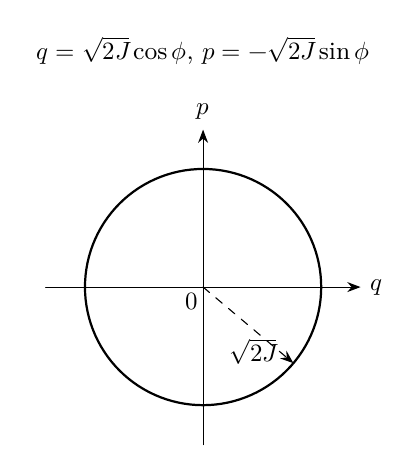
\begin{tikzpicture}[>=Stealth,font=\small,line cap=round,line join=round]
\draw[->,thin] (-2,0) -- (2,0) node[pos=1,right] {$q$};
\draw[->,thin] (0,-2) -- (0,2) node[pos=1,above] {$p$};
\node at (-0.14,-0.18) {$0$};
\draw[thick] plot coordinates {(1.50000,-0.00000) (1.49794,-0.07850) (1.49178,-0.15679) (1.48153,-0.23465) (1.46722,-0.31187) (1.44889,-0.38823) (1.42658,-0.46353) (1.40037,-0.53755) (1.37032,-0.61010) (1.33651,-0.68099) (1.29904,-0.75000) (1.25801,-0.81696) (1.21353,-0.88168) (1.16572,-0.94398) (1.11472,-1.00370) (1.06066,-1.06066) (1.00370,-1.11472) (0.94398,-1.16572) (0.88168,-1.21353) (0.81696,-1.25801) (0.75000,-1.29904) (0.68099,-1.33651) (0.61010,-1.37032) (0.53755,-1.40037) (0.46353,-1.42658) (0.38823,-1.44889) (0.31187,-1.46722) (0.23465,-1.48153) (0.15679,-1.49178) (0.07850,-1.49794) (0.00000,-1.50000) (-0.07850,-1.49794) (-0.15679,-1.49178) (-0.23465,-1.48153) (-0.31187,-1.46722) (-0.38823,-1.44889) (-0.46353,-1.42658) (-0.53755,-1.40037) (-0.61010,-1.37032) (-0.68099,-1.33651) (-0.75000,-1.29904) (-0.81696,-1.25801) (-0.88168,-1.21353) (-0.94398,-1.16572) (-1.00370,-1.11472) (-1.06066,-1.06066) (-1.11472,-1.00370) (-1.16572,-0.94398) (-1.21353,-0.88168) (-1.25801,-0.81696) (-1.29904,-0.75000) (-1.33651,-0.68099) (-1.37032,-0.61010) (-1.40037,-0.53755) (-1.42658,-0.46353) (-1.44889,-0.38823) (-1.46722,-0.31187) (-1.48153,-0.23465) (-1.49178,-0.15679) (-1.49794,-0.07850) (-1.50000,-0.00000) (-1.49794,0.07850) (-1.49178,0.15679) (-1.48153,0.23465) (-1.46722,0.31187) (-1.44889,0.38823) (-1.42658,0.46353) (-1.40037,0.53755) (-1.37032,0.61010) (-1.33651,0.68099) (-1.29904,0.75000) (-1.25801,0.81696) (-1.21353,0.88168) (-1.16572,0.94398) (-1.11472,1.00370) (-1.06066,1.06066) (-1.00370,1.11472) (-0.94398,1.16572) (-0.88168,1.21353) (-0.81696,1.25801) (-0.75000,1.29904) (-0.68099,1.33651) (-0.61010,1.37032) (-0.53755,1.40037) (-0.46353,1.42658) (-0.38823,1.44889) (-0.31187,1.46722) (-0.23465,1.48153) (-0.15679,1.49178) (-0.07850,1.49794) (-0.00000,1.50000) (0.07850,1.49794) (0.15679,1.49178) (0.23465,1.48153) (0.31187,1.46722) (0.38823,1.44889) (0.46353,1.42658) (0.53755,1.40037) (0.61010,1.37032) (0.68099,1.33651) (0.75000,1.29904) (0.81696,1.25801) (0.88168,1.21353) (0.94398,1.16572) (1.00370,1.11472) (1.06066,1.06066) (1.11472,1.00370) (1.16572,0.94398) (1.21353,0.88168) (1.25801,0.81696) (1.29904,0.75000) (1.33651,0.68099) (1.37032,0.61010) (1.40037,0.53755) (1.42658,0.46353) (1.44889,0.38823) (1.46722,0.31187) (1.48153,0.23465) (1.49178,0.15679) (1.49794,0.07850) (1.50000,0.00000)};
\draw[->,thin,dashed] (0,0) -- (1.1472632809267327,-0.9663265308565365) node[pos=0.55,below] {$\sqrt{2J}$};
\node at (0,3) {$q=\sqrt{2J}\cos\phi$, $p=-\sqrt{2J}\sin\phi$};

\end{tikzpicture}
\end{document}
